\section{Specifiche del prodotto}
	I contenuti della specifica saranno presentati seguendo l'approccio top-down: dalla descrizione macroscopica del sistema si scenderà sempre più in dettaglio passando alla descrizione delle singole componenti. Verranno inoltre descritti i design pattern utilizzati e come essi sono stati applicati. Per agevolare la comprensione si è scelto di utilizzare i diagrammi dei package, delle classi, di attività e di sequenza, descritti attraverso lo standard UML 2.0.
	
	\subsection{Architettura generale del sistema}
	Il sistema Quizzipedia è di tipo \emph{client-server}; il \emph{client} fornisce all'utente un'interfaccia web su browser per la creazione e fruizione di questionari, mentre il lato \emph{server} si occupa di gestire e salvare i dati su DBMS MongoDB. La base di dati raccoglie quesiti memorizzati in QML, che su richiesta verranno elaborati da un interprete, questionari (insiemi di quesiti) e i dati degli utenti registrati nel sistema.
Il suddetto interprete processa l'input QML, precedentemente validato nella forma da un parser apposito, traducendolo in linguaggio HTML5 visualizzabile da browser. Il sistema verrà sviluppato utilizzando il framework full-stack Meteor, adottando AngularJS come tecnologia per il rendering e il data-binding dei componenti dell'interfaccia utente.
Nella realizzazione di \emph{Quizzipedia} verrà adottato il design pattern \emph{Model View ViewModel}.
\begin{figure}[h!]
\begin{center}
	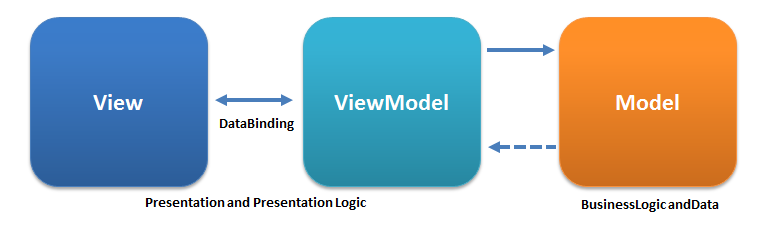
\includegraphics[scale=0.8]{../images/mvvm.png}
	\caption{Il design pattern Model View ViewModel}
\end{center}
\end{figure}
\begin {itemize}
\item\textbf{Model}: definisce l'organizzazione dei dati e ne specifica le modalità di accesso. Nel sistema Quizzipedia è situato nella parte server che opera sulla sottostante base di dati. Fa parte del Model anche la componente \emph{Parser} che opera sui dati prima che essi vengano salvati nel DBMS.
\item\textbf{View}: rappresenta l'interfaccia grafica presentata all'utilizzatore, la quale visualizza i dati e cattura le interazioni dell'utente. Nel pattern \emph{MVVM} è puramente dichiarativa, definita attraverso linguaggi di markup. 
\item\textbf{ViewModel}: è la proiezione di una parte del Model per una View; realizza il data-binding con gli elementi della View e implementa la logica dell'applicazione. 
Realizza il disaccoppiamento totale dalla componente View dal Model.
	\end {itemize}
	Altre possibili architetture sono state prese in considerazione, ma i framework scelti, pensati per la creazione di applicazioni single-page reattive, hanno indirizzato la scelta verso il pattern \emph{MVVM}, che si adatta particolarmente all'utilizzo di AngularJS e al sistema di comunicazione client-server implementato da Meteor (publish-subscribe).

	\subsection{Descrizione del componente Model}
	Il Model, situato nella parte server del sistema svolge le seguenti funzioni:
	\begin{itemize}
		\item Interagisce con un database PostgreSQL nel quale vengono salvati i dati del sistema (ad es. domande, statistiche, utenti). Fornisce quindi adeguate funzionalità di salvataggio e caricamento da database di tali dati.
		\item Al momento del salvataggio di una nuova domanda esegue il \emph{parsing} del codice QML tramite un componente chiamato \emph{Parser}. Se la domanda è sintatticamente corretta può essere salvata nel database.
		\item Offre un'interfaccia logica di accesso al Presenter attraverso la quale richiedere dati e operazioni su di essi.
	\end{itemize}
	\subsection{Descrizione del componente View}
	La componente View rappresenta l'interfaccia grafica che visualizza i dati del Model e inoltra i comandi dell'utente (o gli eventi da esso generati) al Presenter che si occuperà di gestire tali richieste sui dati interagendo col Model; la View si occupa quindi solamente della rappresentazione grafica dei dati e non ha alcun contatto diretto con essi. Essendo un'interfaccia web verrà realizzata tramite HTML5 e CSS3 per le parti statiche e con l'utilizzo di Javascript per le parti dinamiche. Per assicurare uno stile coerente tra le pagine web e migliorare l'adattabilità a piattaforme mobile verrà utilizzato il framework \emph{Materialize}.
	\subsection{Descrizione del componente Presenter}
	Il Presenter ricopre tre ruoli fondamentali: recepire ed elaborare gli input dell'utente,
comunicare col Model, ed aggiornare il View con i dati ottenuti. Per poterlo fare possiede le seguenti caratteristiche:
	\begin{itemize}
		\item Conosce i riferimenti alle altre due componenti. Il Presenter è l'unica componente che conosce entrambe le altre e facendo da singolo tramite tra Model e View permette il loro totale disaccoppiamento;
		\item E' in grado di elaborare gli input della View e tradurli in azioni sul Model. Viceversa ad ogni modifica del Model si preoccupa di aggiornare di conseguenza la View.  
		\item E' responsabile della traduzione delle domande dal formato QML a formato HTML visualizzabile da browser, tramite un componente \emph{Interpreter}.  Tale funzionalità viene richiesta ogni qualvolta il Presenter richiede e riceve dal Model una domanda in formato QML.
		\item Possiede dei gestori che possano modificare l'aspetto della View in reazione all'interazione dell'utente o ai dati ricevuti dal Model. Al suo interno il Presenter contiene delle classi che in risposta ad un evento, quale l'interazione dell'utente con la View o il ricevimento di una risposta dal Model, modificano l'aspetto della GUI presentata.
		\item Gestisce la somministrazione di un questionario ad un utente, domanda dopo domanda, fino alla consegna e valutazione.
	\end{itemize}
	\newpage